\section[Самые сложные задачи]{4. Difficult Problems}

\begin{frame} \frametitle{Карфаген\quad{\it\normalsize (Широкий не значит высокий)}}
\usl{2019-8-1C}{Докажите, что максимальная возможная площадь $n$-угольника, все стороны которого имеют длину 1, меньше, чем максимальная возможная площадь $n+1$-угольника, все стороны которого имеют длину 1.} \vspace{4mm}

Дети же не знают, что максимальную площадь имеют \\
правильные $n$-угольники. \ps

Для каждого многоугольника с $n$ сторонами длины 1 построим многоугольник с $n+1$ сторонами, площадь которого больше.
\end{frame}

\begin{frame} \frametitle{Карфаген\quad{\it\normalsize (Широкий не значит высокий)}}

\begin{center}
\begin{tabular}{ccc}
Если выпуклый & & Если невыпуклый \\
\makecell[c]{
	\definecolor{carthfill}{RGB}{223,223,223}
	\tikz[scale=0.48]{
		\draw[thick] (-1,0) -- ++(60:2) -- (1,0) -- cycle;
		\filldraw[thick,fill=carthfill] (-1,0) ++(195:2) ++(210:2) --
		    ++(30:2) -- ++(15:2) -- ++(0:2) --
		    ++(-15:2) -- ++(-30:2);}
} & \hspace{0.6cm} &
\makecell[c]{
	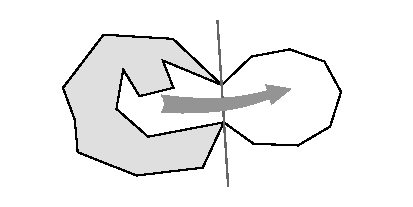
\includegraphics[scale=1.12]{img/carthage}
}
\end{tabular}\end{center}
\end{frame}

\begin{frame} \frametitle{Сортировка}

Выпишем все числа от одного до десяти — но не в привычном порядке возрастания, а в алфавитном порядке: восемь, два, девять, десять, один, пять, семь, три, четыре, шесть. \medskip

\usl{2020-6-4B}{
Числа от 1 до 10'000'000'000 (десять миллиардов) выписали в алфавитном порядке. Перечислите первые десять из них.
}

(1) 18 (2) 18 миллионов (3) 18 миллионов 18 (4) 18 миллионов 18 тысяч \\
(5) 18 миллионов 18 тысяч 18 (6) \ldots восемь (7) \ldots восемьдесят \\
(8) \ldots 88 (9) \ldots 82 (10) \ldots 89.

\end{frame}
